% =========================================================================
% CHAPTER 1: INTRODUCTION
% =========================================================================


\section{Background}
Energy is one of the fundamental pillars of modern society, driving economic growth, industrial development, technological advancement, and improving the quality of life. With the continuous growth of the global population and the rapid expansion of industrialization and urbanization, the demand for electricity has increased significantly in the past several decades. This growing demand has created major challenges in ensuring a reliable, sustainable, and environmentally friendly energy supply.

Traditionally, electricity generation has relied heavily on conventional energy resources such as coal, petroleum, and natural gas. Although fossil fuels have long been the primary source of global electricity generation, their extensive use has resulted in serious environmental challenges. The combustion of fossil fuels releases greenhouse gasses, particularly carbon dioxide (CO2), contributing to global warming, climate change, and air pollution.
In addition, fossil fuel reserves are finite, raising concerns about future energy security.

To address these challenges, the global energy sector has increasingly shifted toward renewable energy resources, which provide clean and sustainable alternatives to conventional energy sources. Consequently, governments, researchers, and industries have invested significant efforts in developing renewable energy technologies and integrating them into
modern electrical power systems.

Among the various renewable energy resources, solar energy has emerged as one of the most promising solutions due to its abundance, accessibility, and minimal environmental impact. The development of photovoltaic (PV) technology has enabled the direct conversion of solar radiation into electrical energy without harmful emissions during operation.
Continuous improvements in photovoltaic materials and manufacturing technologies have enhanced system efficiency while reducing installation costs, making PV systems suitable for residential, commercial, industrial, and utility-scale applications. Today, photovoltaic systems are among the fastest-growing renewable energy technologies worldwide. Their widespread deployment is expected to play a vital role in achieving sustainable development goals, reducing dependence on fossil fuels, and meeting
the growing global demand for clean, reliable, and sustainable electrical energy\cite{masters2013}.

\section{Problem Statement}
The continuous increase in electricity demand has placed considerable pressure on existing power generation systems. Conventional energy resources, which have been the dominant source of electricity production for decades, are associated with several challenges, including limited availability, fluctuating fuel prices, greenhouse gas emissions, and environmental degradation. These issues have raised concerns regarding the ability of current energy systems to satisfy future energy demands in a sustainable manner.

Moreover, many regions around the world continue to experience difficulties in providing reliable electricity due to increasing consumption, population growth, and the depletion of non-renewable energy resources. These challenges highlight the necessity of adopting cleaner, more efficient, and sustainable energy generation technologies that can reduce environmental impacts while maintaining energy security.

Therefore, it has become essential to investigate modern energy solutions capable of meeting the growing electricity demand while minimizing dependence on conventional energy resources. This study contributes to this objective by exploring one of the most promising technologies for sustainable electricity generation.


\section{Renewable Energy}
Renewable energy has become an essential component of modern power systems due to its ability to provide clean and sustainable energy while reducing the environmental impacts associated with conventional energy resources. The increasing global demand for electricity, together with growing concerns about climate change and energy security, has accelerated the development and deployment of renewable energy technologies. Today, renewable energy is widely utilized in residential, commercial, industrial, and utility-scale applications, contributing significantly to the transition toward a more sustainable energy sector.

\subsection{Definition of Renewable Energy}
Renewable energy is defined as energy derived from natural resources that are continuously replenished through natural processes. Unlike fossil fuels, which require millions of years to form and exist in finite quantities, renewable resources are naturally regenerated and can provide a continuous supply of energy when properly utilized. The primary renewable energy resources include solar energy, wind energy, hydropower, biomass, and geothermal energy.

These resources are converted into electrical or thermal energy using different energy conversion technologies. For instance, photovoltaic systems convert solar radiation directly into electricity, while wind turbines convert the kinetic energy of moving air into electrical power. Similarly, hydropower plants utilize the potential and kinetic energy of flowing water to drive turbines connected to electrical generators.


\subsection{Importance of Renewable Energy}
Renewable energy plays a crucial role in addressing many of the challenges facing modern energy systems. It contributes to reducing greenhouse gas emissions, improving air quality, and decreasing dependence on conventional fossil fuels. Furthermore, renewable energy enhances energy security by utilizing locally available natural resources, thereby reducing the need for imported fuels and increasing the stability of national energy supplies.
In addition to its environmental and economic benefits, renewable energy supports sustainable development by promoting technological innovation, creating employment opportunities, and expanding access to electricity, particularly in remote and rural regions.


\begin{figure}[H]
    \centering
    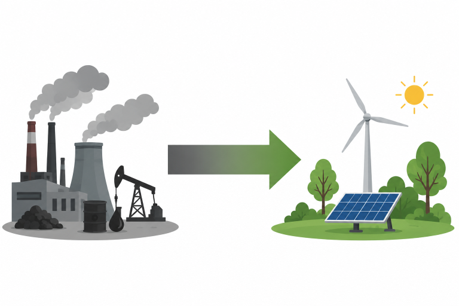
\includegraphics[width=0.75\textwidth]{Figures/Figure 1.1.png}
    \caption{Transition from conventional energy systems to renewable energy systems.}
    \label{fig:energy_transition}
\end{figure}

\subsection{Benefits of Renewable Energy}
Renewable energy provides numerous advantages that make it an attractive alternative to conventional energy resources. It significantly reduces carbon emissions during electricity generation, minimizes environmental pollution, and relies on naturally replenished resources. Moreover, renewable energy systems require relatively low operating and maintenance costs after installation and contribute to improving the diversity and reliability of electrical power systems.

\subsection{Limitations of Renewable Energy}
Despite its numerous advantages, renewable energy technologies still face several technical and economic challenges. The availability of renewable resources often depends on weather conditions and geographical location, resulting in intermittent power generation. Furthermore, the integration of renewable energy into electrical grids requires advanced energy storage technologies, intelligent control systems, and substantial initial investments to ensure reliable and continuous electricity supply.

\section{Renewable Energy Sources}
Renewable energy can be harnessed from various natural resources that are continuously replenished through natural processes. These resources differ in terms of availability, energy conversion methods, efficiency, and practical applications. However, they all share the common objective of providing sustainable energy while reducing dependence on conventional fossil fuels. The primary renewable energy resources include solar energy, wind energy, hydropower, biomass energy, and geothermal energy, each contributing to the diversification of the global energy portfolio.

\begin{figure}[H]
    \centering
    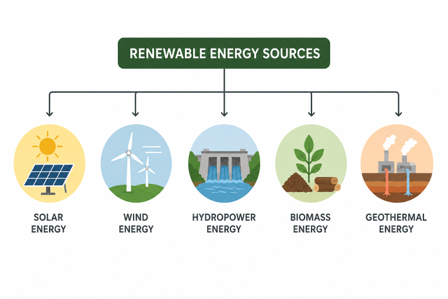
\includegraphics[width=0.75\textwidth]{Figures/Figure 1.2.png}
    \caption{Classification of renewable energy sources.}
    \label{fig:renewable_classification}
\end{figure}

\subsection{Solar Energy}
Solar energy is the energy obtained from solar radiation emitted by the sun. It is considered one of the most abundant and widely available renewable energy resources and can be converted into electrical or thermal energy using different technologies. Owing to its widespread availability and continuous technological development, solar energy has become one of the fastest-growing renewable energy resources worldwide.

\subsection{Wind Energy}
Wind energy utilizes the kinetic energy of moving air to generate electricity through wind turbines. It is a clean and sustainable source of energy that is widely implemented in regions with favorable wind conditions, particularly in coastal and open-land areas.

\subsection{Hydropower}
Hydropower converts the potential and kinetic energy of flowing or falling water into electrical energy using hydraulic turbines. It is one of the oldest and most established renewable energy technologies and is widely used for large-scale electricity generation.

\subsection{Biomass Energy}
Biomass energy is produced from organic materials such as agricultural residues, forestry waste, and other biodegradable resources. These materials can be converted into electricity, heat, or bio-fuels through various biological and thermochemical processes.

\subsection{Geothermal Energy}
Geothermal energy utilizes the thermal energy stored beneath the Earth’s surface for electricity generation and heating applications. It provides a stable and reliable source of energy in regions with suitable geothermal resources.

\section{Solar Energy}
Although several renewable energy resources are available for electricity generation, solar energy has emerged as one of the most promising and widely adopted energy sources due to its abundance, sustainability, and continuous technological advancements. Solar radiation is available in most regions of the world and can be efficiently converted into useful energy using modern conversion technologies.

In particular, countries located within the global sunbelt region, including Egypt, receive high levels of solar irradiance throughout the year, making solar energy an attractive option for electricity generation. As a result, solar energy has become a fundamental component of modern sustainable energy systems and has found extensive applications in residential, commercial, industrial, and transportation sectors.

\subsection{Solar Radiation}
Solar radiation is the electromagnetic energy emitted by the sun as a result of continuous nuclear fusion reactions occurring within its core. This energy propagates through space and reaches the Earth’s atmosphere, where a portion is reflected back into space, another portion is absorbed by atmospheric gases and clouds, while the remaining radiation reaches the Earth’s surface and becomes available for energy conversion.

The amount of solar radiation received at a specific location depends on several factors, including geographical latitude, season of the year, atmospheric conditions, and time of day. Consequently, solar energy availability varies from one region to another, directly influencing the performance of solar energy systems.

Solar radiation reaching the Earth’s surface is generally classified into three main components: direct radiation, diffuse radiation, and reflected radiation. Direct radiation reaches the Earth’s surface without atmospheric scattering, diffuse radiation is scattered by molecules and particles within the atmosphere, whereas reflected radiation originates from sunlight reflected by surrounding objects and the ground. The combination of these components is referred to as global solar radiation, which represents the total solar energy available for solar energy conversion systems.


\begin{figure}[H]
    \centering
    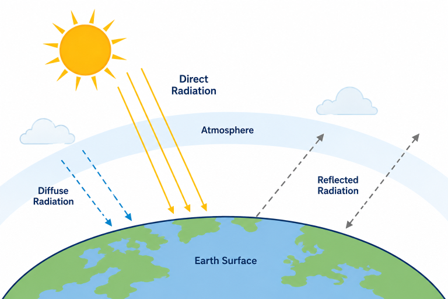
\includegraphics[width=0.75\textwidth]{Figures/Figure 1.3.png}
    \caption{Solar radiation reaching the Earth’s surface.}
    \label{fig:solar_radiation}
\end{figure}


\subsection{Applications of Solar Energy}
The unique characteristics of solar energy have enabled its utilization in a wide range of applications across residential, commercial, industrial, and agricultural sectors. Depending on the required form of energy, solar energy can be employed to provide electricity, heating, and power for remote locations where access to conventional energy sources is limited.

One of the most common applications of solar energy is electricity generation for residential and commercial buildings, where it contributes to reducing dependence on conventional power grids and lowering greenhouse gas emissions. Solar energy is also widely utilized for street lighting, water pumping and irrigation systems, telecommunication stations, and rural electrification projects, providing reliable energy in isolated areas.

In addition, the rapid growth of the transportation sector has created new opportunities for solar energy utilization. The increasing adoption of electric vehicles has encouraged the development of solar-powered charging solutions, supporting the transition toward sustainable transportation while reducing dependence on fossil fuels. As a result, solar energy has become an essential component of modern clean energy systems.


\begin{figure}[H]
    \centering
    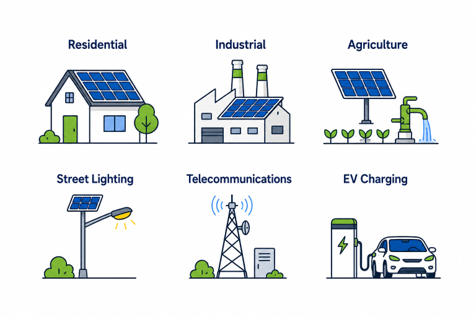
\includegraphics[width=0.75\textwidth]{Figures/Figure 1.4.png}
    \caption{Various applications of solar energy.}
    \label{fig:solar_applications}
\end{figure}

\subsection{Advantages and Challenges of Solar Energy}
Solar energy has become one of the most attractive renewable energy resources due to its environmental, economic, and technical benefits. It is an abundant and inexhaustible source of energy that is naturally replenished and available in most regions of the world. During operation, solar energy systems produce electricity without emitting greenhouse gases or air pollutants, contributing to environmental protection and climate change mitigation. In addition, solar energy systems generally require low operating and maintenance costs and can be deployed at various scales, ranging from small residential installations to large utility-scale power plants.

Despite these advantages, several challenges still limit the widespread utilization of solar energy. The amount of energy generated depends on solar irradiance, which varies according to weather conditions, seasonal changes, and the time of day. Consequently, electricity generation is intermittent and unavailable during nighttime. Moreover, the relatively high initial installation cost and the need for efficient energy storage technologies remain important considerations in solar energy systems. Continuous technological developments are therefore focused on improving system efficiency, reducing installation costs, and enhancing the reliability of solar energy utilization.


\section{Photovoltaic Systems}
Although solar energy is an abundant and sustainable source of renewable energy, it must be converted into electrical energy before it can be utilized in most practical applications. This conversion is achieved using photovoltaic (PV) technology, which directly transforms solar radiation into electricity through semiconductor materials. Owing to its high efficiency, reliability, and environmental benefits, photovoltaic technology has become one of the fastest-growing electricity generation technologies worldwide and plays a fundamental role in modern renewable energy systems.

\subsection{History and Development of Photovoltaic Technology}
The history of photovoltaic (PV) technology began in 1839 when the French physicist Alexandre Edmond Becquerel discovered the photovoltaic effect while conducting experiments on metal electrodes immersed in an electrolyte solution exposed to sunlight. His discovery demonstrated, for the first time, that light energy could be directly converted into electrical energy, laying the scientific foundation for modern photovoltaic technology.

The first practical attempt to utilize this phenomenon was made in 1883 by the American inventor Charles Fritts, who developed the first selenium-based solar cell. Although its energy conversion efficiency was relatively low, this achievement represented the first successful implementation of photovoltaic energy conversion and marked an important milestone in the evolution of solar cell technology.

A major breakthrough was achieved in 1954 when researchers at Bell Laboratories developed the first practical silicon solar cell with significantly higher conversion efficiency, making photovoltaic technology suitable for real-world applications. A few years later, in 1958, photovoltaic cells were successfully employed to power the Vanguard 1 satellite, demonstrating their exceptional reliability and establishing photovoltaics as a preferred energy source for space applications.

Since then, continuous advancements in semiconductor materials, manufacturing techniques, and power electronic technologies have significantly improved the efficiency, durability, and cost-effectiveness of photovoltaic systems. These developments have enabled the widespread deployment of PV systems in residential, commercial, industrial, and utility-scale electricity generation. Today, photovoltaic technology has become one of the leading renewable energy technologies for clean and sustainable electricity production worldwide.


\begin{figure}[H]
    \centering
    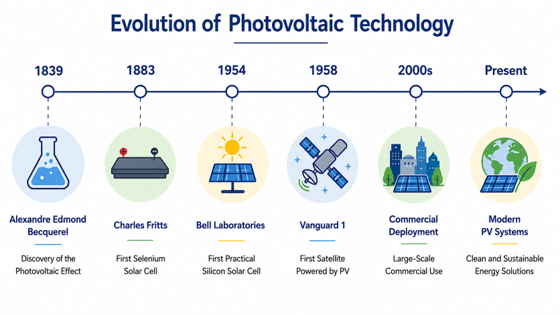
\includegraphics[width=0.85\textwidth]{Figures/Figure 1.5.png}
    \caption{Major milestones in the development of photovoltaic technology.}
    \label{fig:pv_history}
\end{figure}

\newpage

\subsection{Photovoltaic System Components}
Photovoltaic (PV) systems consist of several interconnected components that work together to convert solar energy into usable electrical power. The basic building block of every photovoltaic system is the photovoltaic cell, which converts sunlight directly into electricity through the photovoltaic effect. To satisfy practical power requirements, individual cells are electrically interconnected to form modules, while multiple modules are combined into arrays capable of generating higher voltage and power levels. In addition to the photovoltaic array, a complete PV system includes several auxiliary components, collectively referred to as the Balance of System (BOS), which ensure efficient energy conversion, control, protection, and power delivery.

\subsubsection{Photovoltaic Cell}
A photovoltaic (PV) cell is the fundamental building block of every photovoltaic system and is the smallest unit capable of directly converting solar energy into electrical energy through the photovoltaic effect. It is typically fabricated from semiconductor materials, with crystalline silicon being the most widely used due to its high efficiency, reliability, and long operational lifetime. A single photovoltaic cell generates a relatively small electrical output, typically around 0.5–0.7 V under standard test conditions (STC), making it necessary to electrically connect multiple cells to obtain practical voltage and power levels.

\begin{figure}[H]
    \centering
    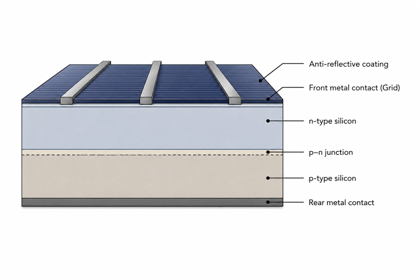
\includegraphics[width=0.65\textwidth]{Figures/Figure 1.6.png}
    \caption{Cross-sectional structure of a photovoltaic cell.}
    \label{fig:pv_cell_structure}
\end{figure}

The structure of a photovoltaic cell is carefully designed to maximize sunlight absorption while minimizing electrical losses. The front surface is covered with an anti-reflective coating to reduce optical reflection and increase the amount of incident solar radiation entering the semiconductor. Metallic contacts are provided on both the front and rear surfaces to collect the generated charge carriers and transfer the electrical current to the external circuit. These structural components enable efficient energy conversion and provide the foundation for larger photovoltaic modules and arrays.

\subsubsection{Photovoltaic Module}
Since the electrical output of a single photovoltaic cell is relatively low, multiple photovoltaic cells are electrically interconnected to form a photovoltaic module. The cells are typically connected in series to increase the output voltage, while parallel connections are used when higher current is required. The interconnected cells are encapsulated between protective layers, including tempered glass, polymer encapsulant materials, and a durable backsheet, to provide mechanical strength and protect the cells from environmental conditions such as moisture, dust, and temperature variations.

\begin{figure}[H]
    \centering
    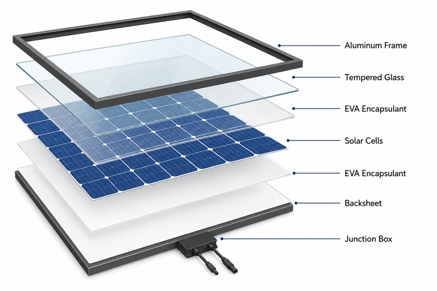
\includegraphics[width=0.65\textwidth]{Figures/Figure 1.7.png}
    \caption{Exploded view of a photovoltaic module showing its main structural components.}
    \label{fig:pv_module_exploded}
\end{figure}

Photovoltaic modules are manufactured in standardized sizes and power ratings to facilitate system design and installation. Depending on the application, modules can be connected together in various electrical configurations to achieve the required voltage, current, and power output. As the primary structural unit of a photovoltaic array, modules provide a practical balance between electrical performance, mechanical durability, and ease of maintenance.

\subsubsection{Photovoltaic Array}
A photovoltaic array consists of multiple photovoltaic modules electrically interconnected to provide the voltage, current, and power required for a specific application. The modules may be connected in series to increase the output voltage or in parallel to increase the output current. In practical PV installations, a combination of series and parallel connections is commonly employed to achieve the desired electrical characteristics while meeting the system’s power demand.

The electrical output of a photovoltaic array depends on several operating conditions, including solar irradiance, cell temperature, shading, and the electrical configuration of the modules. By adjusting the number of modules connected in series and parallel, PV arrays can be designed to satisfy a wide range of residential, commercial, and industrial energy requirements. Consequently, the photovoltaic array represents the primary power-generating unit within a photovoltaic system.

\begin{figure}[H]
    \centering
    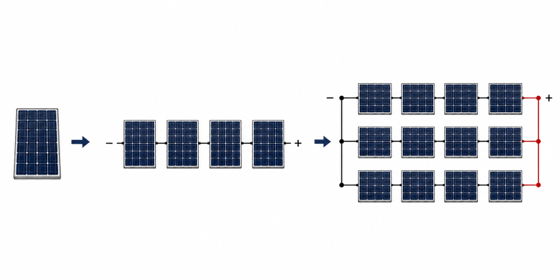
\includegraphics[width=0.75\textwidth]{Figures/Figure 1.8.png}
    \caption{Formation of a photovoltaic array from modules connected in series and parallel.}
    \label{fig:pv_array_formation}
\end{figure}


\subsubsection{Balance of System (BOS)}
In addition to photovoltaic modules and arrays, a complete photovoltaic system requires several auxiliary components collectively known as the Balance of System (BOS). These components are responsible for controlling, protecting, converting, storing, and delivering the generated electrical energy. Although they do not directly generate electricity, BOS components play a crucial role in ensuring the safe, reliable, and efficient operation of the entire photovoltaic system.

\subsection{Operating Principle of Photovoltaic Systems}
The operation of a photovoltaic (PV) system begins when solar radiation reaches the surface of a photovoltaic cell. Sunlight consists of tiny packets of energy known as photons. As these photons strike the surface of the PV cell, a portion of their energy penetrates the semiconductor material, initiating the energy conversion process. The amount of absorbed solar energy depends on the intensity of solar irradiance and the optical properties of the photovoltaic material.

\begin{figure}[H]
    \centering
    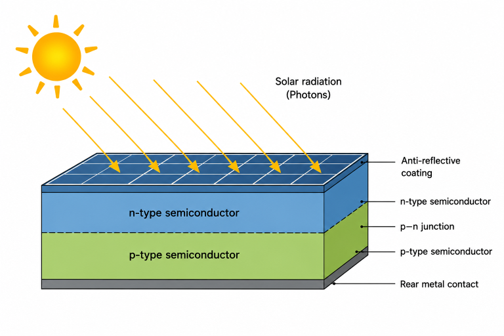
\includegraphics[width=0.55\textwidth]{Figures/Figure 1.9.png}
    \caption{Incident solar radiation on a photovoltaic cell.}
    \label{fig:pv_incident}
\end{figure}

\newpage

When photons penetrate the semiconductor material, they transfer their energy to the electrons bound within the silicon atoms. If the energy of an incident photon is equal to or greater than the band-gap energy of the semiconductor, the electron gains sufficient energy to break free from its atomic bond and move into the conduction band. Consequently, an empty position, known as a hole, is left behind in the valence band. The simultaneous creation of a free electron and a hole is referred to as an electron–hole pair, representing the first step in the generation of electrical energy within a photovoltaic cell.

\begin{figure}[H]
    \centering
    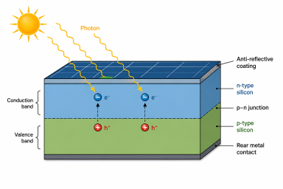
\includegraphics[width=0.55\textwidth]{Figures/Figure 1.10.png}
    \caption{Generation of electron–hole pairs inside a photovoltaic cell.}
    \label{fig:pv_eh_pairs}
\end{figure}

The electron–hole pairs generated within the photovoltaic cell are immediately separated by the built-in electric field established across the p–n junction. This electric field drives the free electrons toward the n-type semiconductor layer, while the holes move toward the p-type layer. By separating the charge carriers, the electric field minimizes their recombination and creates a potential difference across the cell, which is essential for generating electrical power.

\begin{figure}[H]
    \centering
    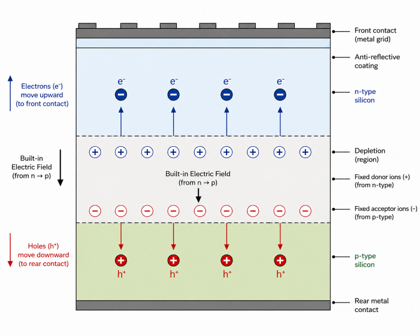
\includegraphics[width=0.55\textwidth]{Figures/Figure 1.11.png}
    \caption{Separation of charge carriers by the built-in electric field.}
    \label{fig:pv_separation}
\end{figure}

\newpage

When an external electrical circuit is connected to the photovoltaic cell, the separated electrons flow through the external circuit from the n-type contact to the p-type contact, producing a direct current (DC). As the electrons pass through the connected electrical load, they deliver useful electrical energy before returning to the photovoltaic cell, where the cycle continues as long as sunlight is available.

\begin{figure}[H]
    \centering
    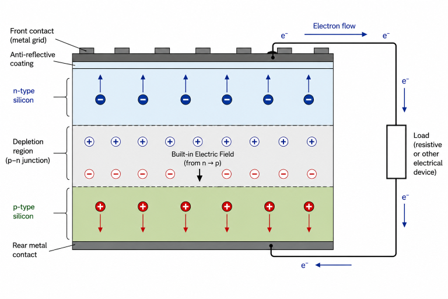
\includegraphics[width=0.55\textwidth]{Figures/Figure 1.12.png}
    \caption{Electron flow through the external circuit producing direct current (DC).}
    \label{fig:pv_current_flow}
\end{figure}

\subsection{Photovoltaic System Configurations}
Photovoltaic systems can be configured using different electrical architectures depending on the required power capacity, system efficiency, reliability, and application requirements. The configuration of a PV system determines how photovoltaic modules are interconnected and how the generated electrical power is processed before being supplied to the load or the utility grid. Among the most common configurations are centralized, string, and multi-string photovoltaic systems, each offering distinct advantages and limitations in terms of performance, flexibility, maintenance, and energy conversion efficiency.

\subsubsection{Centralized Photovoltaic Configuration}
In a centralized photovoltaic configuration, multiple photovoltaic strings are connected to a single central power conversion unit equipped with a common maximum power point tracking (MPPT) controller. This architecture is widely employed in large-scale photovoltaic power plants because of its simple design, reduced installation cost, and ease of implementation. However, since all PV strings operate under a single MPPT controller, the overall system performance can be significantly affected by partial shading, module mismatch, or faults occurring within individual strings. As a result, the entire system operates according to a common operating point rather than the optimum operating point of each individual string, leading to a reduction in the overall energy yield.

\begin{figure}[H]
    \centering
    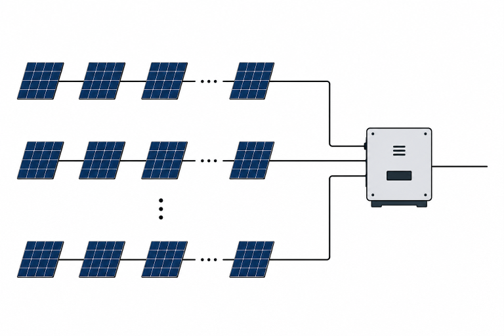
\includegraphics[width=0.65\textwidth]{Figures/Figure 1.13.png}
    \caption{Conceptual illustration of a centralized photovoltaic system configuration.}
    \label{fig:central_config}
\end{figure}

\subsubsection{String Photovoltaic Configuration}
In a string photovoltaic configuration, each photovoltaic string is connected to its own power conversion unit equipped with an independent maximum power point tracking (MPPT) controller. This allows every string to operate independently at its individual maximum power point, thereby improving the overall energy harvest under non-uniform operating conditions. Compared with the centralized configuration, this architecture significantly reduces the impact of partial shading, module mismatch, and string faults on the overall system performance. Consequently, string photovoltaic systems offer higher flexibility, improved reliability, and easier maintenance, making them widely adopted in residential and commercial photovoltaic installations.

\begin{figure}[H]
    \centering
    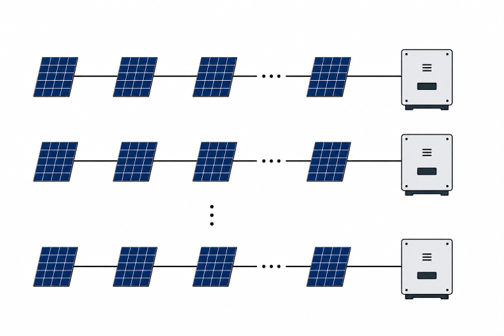
\includegraphics[width=0.65\textwidth]{Figures/Figure 1.14.png}
    \caption{Conceptual illustration of a string photovoltaic system configuration.}
    \label{fig:string_config}
\end{figure}

\newpage

\subsubsection{Multi-String Photovoltaic Configuration}
A multi-string photovoltaic configuration combines the advantages of both centralized and string photovoltaic systems. In this architecture, each photovoltaic string is connected to an individual DC–DC converter equipped with an independent maximum power point tracking (MPPT) controller before being connected to a common DC bus.

This enables each string to operate at its own maximum power point regardless of the operating conditions of the other strings, thereby maximizing the overall energy harvested from the photovoltaic array.
Comparison of the main characteristics of centralized, string, and multi-string photovoltaic system configurations.


\begin{figure}[H]
    \centering
    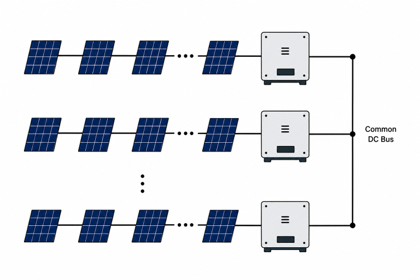
\includegraphics[width=0.65\textwidth]{Figures/Figure 1.15.png}
    \caption{Conceptual illustration of a multi-string photovoltaic system configuration.}
    \label{fig:multistring_config}
\end{figure}

\begin{table}[H]
    \centering
    \caption{Comparison of the main characteristics of centralized, string, and multi-string photovoltaic system configurations.}
    \label{tab:pv_configurations}
    \smallskip
    \smallskip
    \renewcommand{\arraystretch}{1.4} % Nice breathing room between rows
    \rowcolors{2}{white}{gray!8} % Clean alternating zebra stripes
    
    % This customizes the width ratios of your columns perfectly
    \begin{tabularx}{\textwidth}{
        >{\hsize=1.4\hsize\raggedright\arraybackslash}X 
        >{\hsize=0.86\hsize\raggedright\arraybackslash}X 
        >{\hsize=0.86\hsize\raggedright\arraybackslash}X 
        >{\hsize=0.88\hsize\raggedright\arraybackslash}X
    }
        \toprule
        \textbf{Feature} & \textbf{Centralized} & \textbf{String} & \textbf{Multi-String} \\
        \midrule
        Number of MPPT Controllers & One & One per String & One per String \\
        MPPT Operation & Common MPPT & Independent MPPT & Independent MPPT \\
        Power Conversion Architecture & Single Central Converter & One Converter per String & One Converter per String + Common DC Bus \\
        Common DC Bus & No & No & Yes \\
        Partial Shading Performance & Poor & Good & Excellent \\
        Module Mismatch Tolerance & Low & High & Very High \\
        System Reliability & Moderate & High & Very High \\
        Scalability & Limited & Good & Excellent \\
        Maintenance & Difficult & Easy & Easy \\
        Initial Cost & Low & Moderate & Higher \\
        \bottomrule
    \end{tabularx}
\end{table}

Based on the comparison presented in Table 1, the multi-string photovoltaic configuration provides an effective compromise between efficiency, flexibility, and reliability. Owing to these advantages, this configuration has been adopted as the photovoltaic architecture of the proposed system presented in this project.

\newpage

\section{Battery Energy Storage System}
Battery Energy Storage Systems (BESSs) play a vital role in photovoltaic-based energy systems by balancing power generation and demand. They enable excess electrical energy to be stored for later use, thereby improving energy utilization, enhancing system reliability, and maintaining a stable power supply under varying operating conditions\cite{dunn2011}.

\subsection{Overview of Battery Energy Storage Systems}
A (BESS) is an electrochemical energy storage system designed to store electrical energy and release it whenever required. It consists of battery cells, a battery management system (BMS), and associated power electronic components that collectively ensure efficient, safe, and reliable operation.

BESS has become an essential component in renewable energy systems because it improves the flexibility of power management and increases the utilization of generated energy. By balancing the mismatch between energy generation and demand, battery storage systems contribute to maintaining system stability and supporting continuous operation under different operating conditions.

\begin{figure}[H]
    \centering
    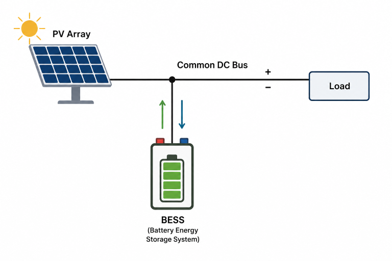
\includegraphics[width=0.65\textwidth]{Figures/Figure 1.16.png}
    \caption{Conceptual integration of a Battery Energy Storage System (BESS) with a common DC bus in a photovoltaic-based energy system.}
    \label{fig:bess_integration}
\end{figure}

\subsection{Operating Principle of Battery Energy Storage Systems}
The operating principle of a Battery Energy Storage System (BESS) is based on reversible electrochemical reactions that enable the storage and release of electrical energy. During the charging process, electrical energy supplied from an external source is converted into chemical energy and stored within the battery cells. During discharging, the stored chemical energy is converted back into electrical energy to supply the connected load.

\begin{figure}[H]
    \centering
    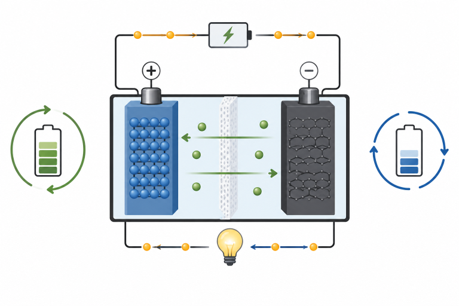
\includegraphics[width=0.65\textwidth]{Figures/Figure 1.17.png}
    \caption{Electrochemical operating principle of a battery energy storage system during charging and discharging processes.}
    \label{fig:bess_electrochemistry}
\end{figure}

The charging and discharging processes are continuously monitored and controlled by the Battery Management System (BMS), which regulates key operating parameters such as voltage, current, temperature, and State of Charge (SOC). Proper battery management improves operational safety, prevents overcharging and excessive discharging, and contributes to extending the battery lifetime while maintaining reliable system performance.

\subsection{Battery Technologies}
Various battery technologies have been developed for energy storage applications, each offering different characteristics in terms of energy density, efficiency, lifetime, cost, and maintenance requirements. The selection of a suitable battery technology depends on the intended application, operating conditions, and system requirements. Among the most widely used battery technologies are lead-acid, nickel-metal hydride (NiMH), and lithium-ion batteries\cite{dunn2011}.

Among the available battery technologies, lithium-ion batteries exhibit the highest energy density, round-trip efficiency, and cycle life. In addition, they offer low maintenance requirements and excellent electrochemical performance, making them the preferred choice for modern photovoltaic energy storage systems despite their relatively higher initial cost.

\begin{table}[H]
    \centering
    \caption{Comparison of Common Battery Technologies.}
    \label{tab:battery_technologies}
    
    \renewcommand{\arraystretch}{1.4} % Nice vertical padding between rows
    \rowcolors{2}{white}{gray!8} % Clean alternating zebra stripes
    
    % Proportional constraints: Gives more room to the first column 
    % and splits the remaining width perfectly across the numerical data columns
    \begin{tabularx}{\textwidth}{
        >{\hsize=1.4\hsize\raggedright\arraybackslash}X 
        >{\hsize=0.9\hsize\raggedright\arraybackslash}X 
        >{\hsize=0.9\hsize\raggedright\arraybackslash}X 
        >{\hsize=0.9\hsize\raggedright\arraybackslash}X
        >{\hsize=0.9\hsize\raggedright\arraybackslash}X
    }
        \toprule
        \textbf{Battery Technology} & \textbf{Energy Density} & \textbf{Efficiency} & \textbf{Cycle Life} & \textbf{Relative Cost} \\
         & \textbf{(Wh/kg)} & \textbf{(\%)} & \textbf{(cycles)} &  \\
        \midrule
        Lead-Acid & 30–50 & 70–85 & 500–1,000 & Low \\
        Nickel-Metal Hydride (NiMH) & 60–120 & 65–80 & 500–2,000 & Moderate \\
        Lithium-Ion & 150–250 & 90–95 & 2,000–7,000 & High \\
        \bottomrule
    \end{tabularx}
\end{table}

\subsection{Lithium-Ion Batteries}
Lithium-ion (Li-ion) batteries are the most widely used rechargeable batteries in modern energy storage applications due to their high energy density, high efficiency, long cycle life, and low self-discharge rate. Compared with conventional battery technologies, lithium-ion batteries provide superior electrochemical performance while requiring minimal maintenance. These characteristics have made them the preferred choice for photovoltaic energy storage systems, electric vehicles, and other applications requiring reliable and efficient energy storage\cite{dunn2011}.

The operation of a lithium-ion battery is based on the movement of lithium ions between the anode and the cathode through the electrolyte. During charging, lithium ions migrate from the cathode to the anode, where they are stored within the electrode material. During discharging, the ions move back to the cathode while electrons flow through the external circuit, delivering electrical energy to the connected load. This reversible electrochemical process enables repeated charging and discharging cycles with high efficiency and excellent energy storage capability.

\begin{figure}[H]
    \centering
    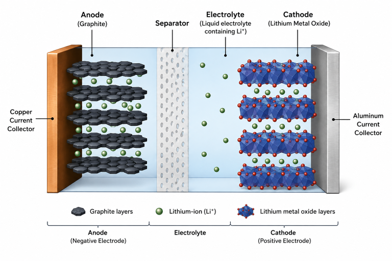
\includegraphics[width=0.7\textwidth]{Figures/Figure 1.18.png}
    \caption{Schematic structure of a lithium-ion battery showing its main components, including the anode, cathode, separator, electrolyte, and current collectors.}
    \label{fig:liion_structure}
\end{figure}
\section{Utility Grid}
The utility grid is an interconnected electrical network responsible for transmitting and distributing electrical power from generation stations to end users. It consists of generation units, high-voltage transmission lines, substations, and distribution networks operating together to ensure reliable, stable, and continuous electricity supply. Modern utility grids are designed to maintain system stability while accommodating continuously varying load demands.
\subsection{Overview of the Utility Grid}
The primary objective of the utility grid is to deliver electrical energy while maintaining stable voltage and frequency within specified operating limits. Electrical power generated at power plants is transmitted over long distances using high-voltage transmission networks to minimize transmission losses before being distributed to consumers through medium- and low-voltage distribution systems. Grid operation is continuously supervised using monitoring, protection, and control systems to ensure secure and reliable power delivery
\begin{figure}[H]
    \centering
    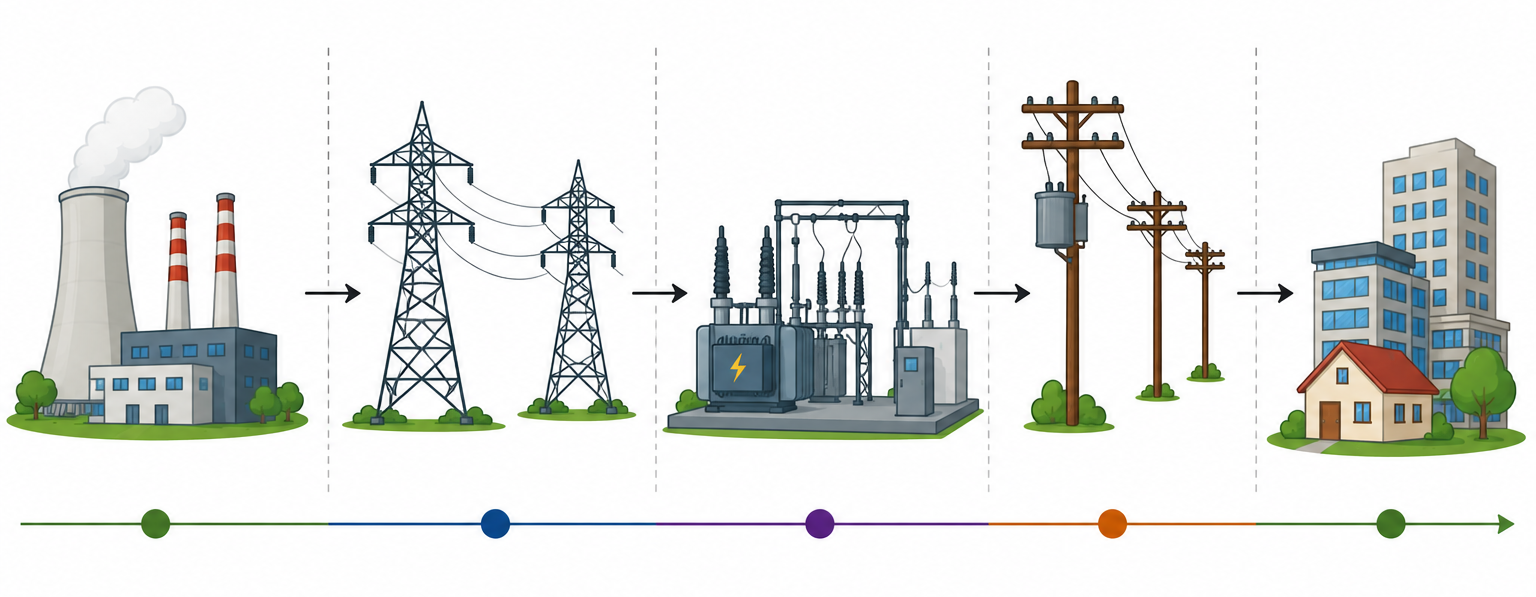
\includegraphics[width=\textwidth]{Figures/Grid .png}
    \caption{General structure of a utility grid illustrating the flow of electrical power from generation to end users through transmission, substations, and distribution networks.}
    \label{fig:utility_grid_structure}
\end{figure}
\subsection{Operating Principle of the Utility Grid}
The operation of the utility grid is based on maintaining a continuous balance between electrical power generation and load demand. Power generated from different generating stations is synchronized and transmitted through interconnected transmission networks before reaching distribution systems and end users. System operators continuously regulate power flow, voltage, and frequency to ensure stable operation under varying loading conditions while maintaining power quality and system reliability.

\newpage
\subsection{Characteristics of Modern Utility Grids}
Modern utility grids are characterized by high reliability, large power transmission capability, and extensive geographical coverage. The integration of advanced monitoring systems, communication technologies, and power electronic converters has significantly improved grid flexibility and operational efficiency. These developments have enabled modern utility grids to accommodate distributed generation, renewable energy sources, and bidirectional power flow while maintaining secure and stable system operation\cite{rehmani2018}.

\section{Electric Vehicle Charging Systems}
Electric vehicles (EVs) have emerged as a promising solution for reducing greenhouse gas emissions and decreasing dependence on fossil fuels. Their rapid global adoption has increased the demand for reliable and efficient charging infrastructure capable of supporting sustainable transportation systems.

\subsection{Overview of Electric Vehicles}
An electric vehicle (EV) is a vehicle powered wholly or partially by electrical energy stored in rechargeable batteries. Unlike conventional internal combustion engine vehicles, electric vehicles use electric motors for propulsion, resulting in higher energy efficiency, lower operating costs, and zero tailpipe emissions. These advantages have accelerated the adoption of electric vehicles in both residential and commercial transportation sectors.

The rapid advancement of battery technologies, continuous improvements in charging infrastructure, and growing environmental awareness have significantly accelerated the global adoption of electric vehicles. As a result, electric vehicles have become a key component of sustainable transportation systems, offering an effective solution for reducing greenhouse gas emissions and improving overall energy efficiency\cite{tie2013,emadi2015}.


\begin{figure}[H]
    \centering
    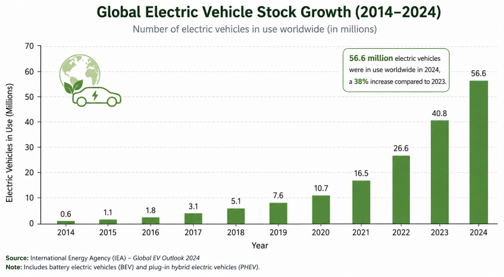
\includegraphics[width=0.75\textwidth]{Figures/Figure 1.19.png}
    \caption{Global growth of electric vehicle stock between 2014 and 2024 (adapted from \cite{iea2024}).}
    \label{fig:ev_growth}
\end{figure}

\newpage

\subsection{Electric Vehicle Charging}
Electric vehicle charging is the process of transferring electrical energy from an external power source to the battery pack of an electric vehicle. The charging process is performed through dedicated charging equipment that safely delivers electrical energy while monitoring charging parameters to ensure reliable and efficient battery operation.

Electric vehicle charging stations can be supplied from different energy sources, including the utility grid, renewable energy systems, or hybrid energy systems. Among these, photovoltaic-powered charging stations have gained considerable attention because they utilize clean solar energy to charge electric vehicles, thereby reducing greenhouse gas emissions and decreasing dependence on conventional electricity generation\cite{tie2013}.

\begin{figure}[H]
    \centering
    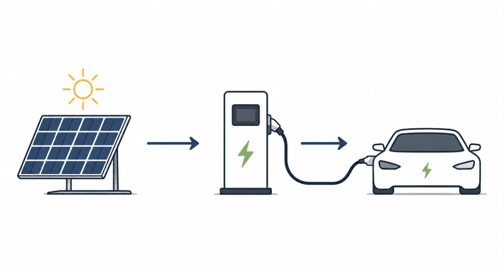
\includegraphics[width=0.65\textwidth]{Figures/Figure 1.20.png}
    \caption{Conceptual illustration of a photovoltaic-powered electric vehicle charging system.}
    \label{fig:pv_ev_charging}
\end{figure}

Depending on the charging power and charging duration, electric vehicle charging systems are generally classified into different charging levels. These charging levels provide various charging speeds to satisfy different user requirements and application scenarios.

\subsection{Electric Vehicle Charging Levels}
Electric vehicle charging systems are commonly classified according to the charging power, supply voltage, and charging duration. Different charging levels have been developed to satisfy various charging requirements ranging from residential overnight charging to rapid public charging stations. The selection of an appropriate charging level depends on factors such as battery capacity, charging time, installation cost, and application requirements.

\begin{table}[H]
    \centering
    \caption{Comparison of Electric Vehicle Charging Levels.}
    \label{tab:charging_levels}
    
    \renewcommand{\arraystretch}{1.4} % Nice vertical padding between rows
    \rowcolors{2}{white}{gray!8} % Clean alternating zebra stripes
    
    % Proportional constraints: Allocates balanced page-width ratios 
    % so that columns wrap text beautifully and fit within your margins
    \begin{tabularx}{\textwidth}{
        >{\hsize=1.1\hsize\raggedright\arraybackslash}X 
        >{\hsize=1.0\hsize\raggedright\arraybackslash}X 
        >{\hsize=0.8\hsize\raggedright\arraybackslash}X 
        >{\hsize=1.0\hsize\raggedright\arraybackslash}X
        >{\hsize=1.1\hsize\raggedright\arraybackslash}X
    }
        \toprule
        \textbf{Charging Level} & \textbf{Supply} & \textbf{Power} & \textbf{Charging Time} & \textbf{Typical Application} \\
        \midrule
        Level 1 & 120 V AC & 1.4–1.9 kW & 8–20 h & Residential \\
        Level 2 & 208–240 V AC & 3.3–22 kW & 2–8 h & Residential / Commercial \\
        DC Fast Charging & 400–1000 V DC & 25–350 kW & 20–60 min & Public Charging Stations \\
        \bottomrule
    \end{tabularx}
\end{table}

As summarized in Table 3, Level 1 charging is mainly intended for overnight residential charging due to its low charging power. Level 2 charging provides a practical balance between charging speed and installation cost, making it suitable for residential and commercial applications. In contrast, DC fast charging delivers significantly higher charging power, enabling rapid battery charging in public charging stations where minimizing charging time is a priority.

\section{Common DC Bus Architecture}
A common DC bus architecture is widely employed in photovoltaic-powered electric vehicle charging systems to integrate multiple energy sources and loads into a unified electrical platform. In this configuration, the photovoltaic (PV) array, battery energy storage system (BESS), utility grid, and electric vehicle (EV) charger are interconnected through a common DC link. The utility grid is interfaced with the DC bus via a bidirectional grid-tied AC/DC converter, enabling controlled power exchange between the charging station and the electrical network. This architecture minimizes unnecessary power conversion stages, improves energy management, and enhances overall system flexibility.
\begin{figure}[H]
    \centering
    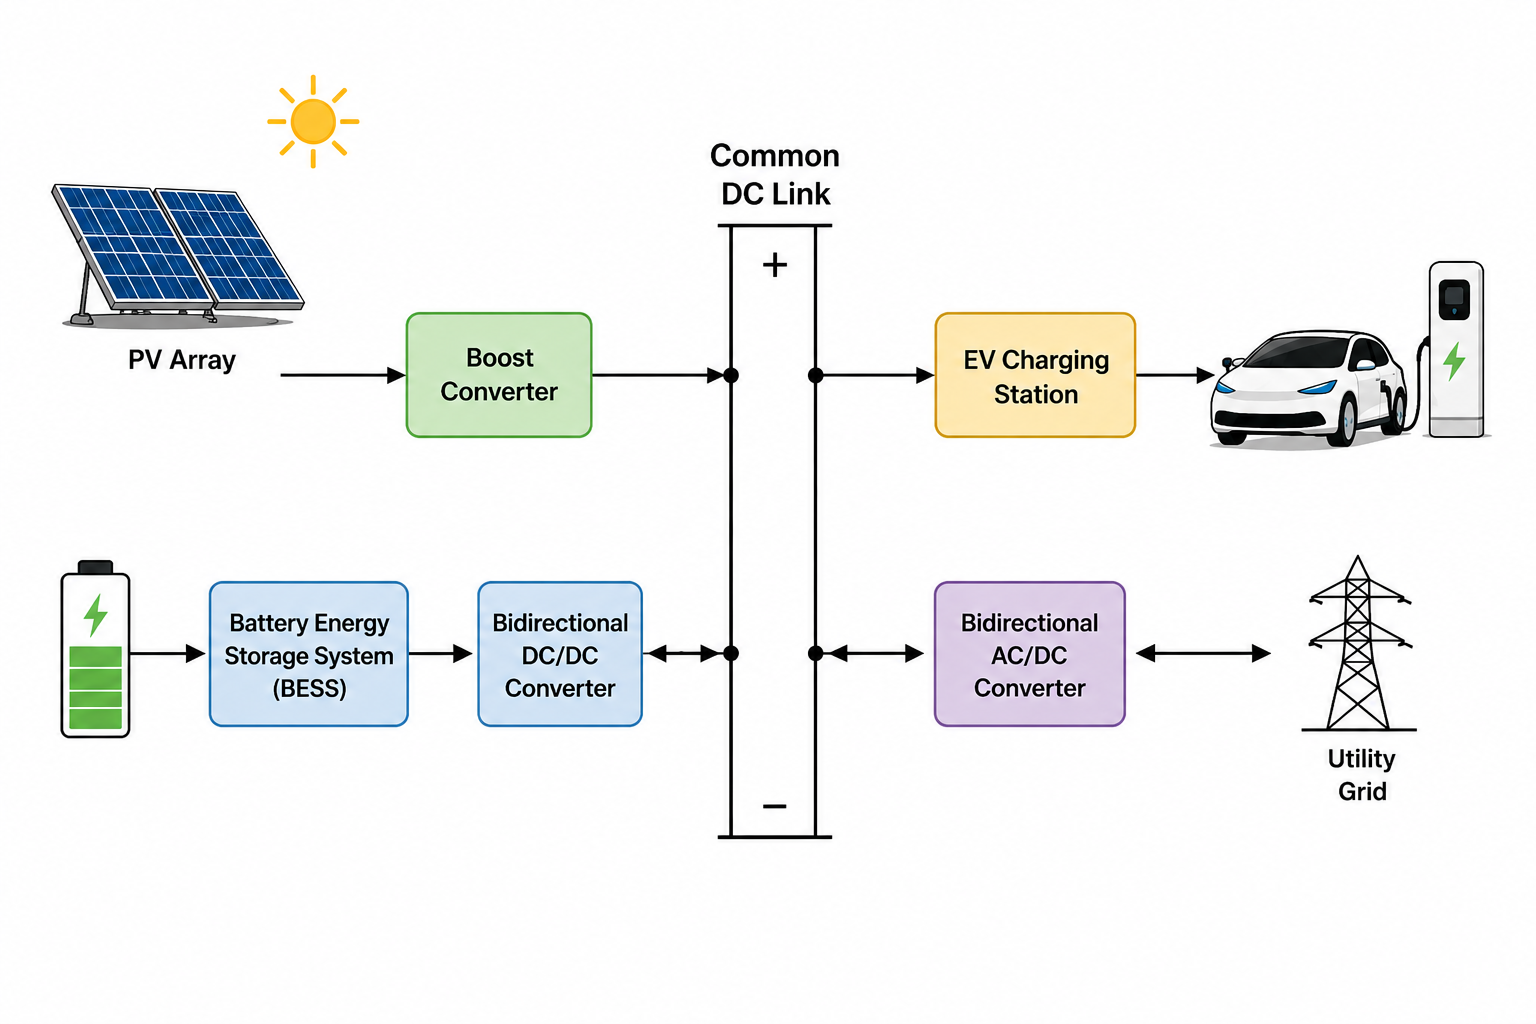
\includegraphics[width=0.9\textwidth]{Figures/system.png}
    \caption{General architecture of a photovoltaic-powered electric vehicle charging system based on a common DC bus.}
    \label{fig:dc_bus_architecture}
\end{figure}
The operating principle of the proposed system is based on coordinated power exchange through the common DC link. Electrical energy generated by the photovoltaic array is boosted to the required DC voltage and supplied to the DC bus. The EV charger draws power directly from the DC link to charge the vehicle battery. The Battery Energy Storage System (BESS) stores excess photovoltaic energy during periods of surplus generation and discharges it when additional power is required. Meanwhile, the utility grid exchanges power with the DC link through a bidirectional AC/DC converter. The grid supplies energy when the available photovoltaic generation and battery storage are insufficient to satisfy the charging demand, while excess energy can be exported back to the utility grid under appropriate operating conditions. This coordinated operation improves power management, increases overall system efficiency, and ensures reliable EV charging under varying operating conditions.
\section{Chapter Summary}
This chapter provided the theoretical background of the proposed photovoltaic-powered electric vehicle charging system. It reviewed the operating principles and essential characteristics of photovoltaic systems, battery energy storage systems, and electric vehicle charging systems. In addition, the common DC bus architecture was introduced to demonstrate the integration and power flow among the system components. This background serves as the foundation for the system design, modeling, control strategy, and simulation results presented in the subsequent chapters.